\documentclass[a4paper,12pt]{article}

\usepackage[right=2cm,top=1cm,left=2cm,bottom=1cm]{geometry}
\usepackage{graphicx}
\usepackage[utf8]{inputenc}
\usepackage[russian]{babel}
\usepackage{fontspec}
\usepackage{listings}

\setmainfont{Liberation Serif}
\lstset{basicstyle=\footnotesize\ttfamily,breaklines=true}

\pagenumbering{gobble}

\title{Практическая работа №15 по дисциплине\\«Языки программирования»\\Изучение механизма простого и множественного наследования}
\author{Сердюков Матвей, БББО-05-19}
\date{Вариант 2}

\begin{document}
	\maketitle
	\section{Схема наследования}
	\begin{figure}[h]
			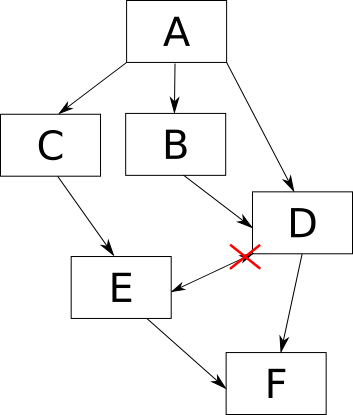
\includegraphics[scale=0.8]{scheme.png}
			\centering
	\end{figure}
	\begin{figure}[h]
			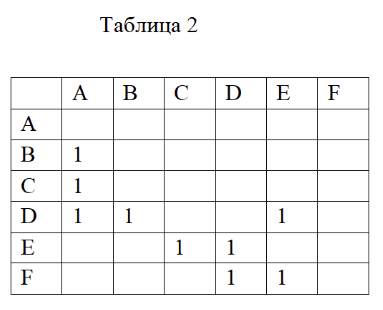
\includegraphics[scale=0.45]{table.png}
			\centering
	\end{figure}
	\noindent
	Согласно таблице наследования, классы D и E наследуются друг от друга, что невозможно. В связи с этим будем игнорировать наследование класса D от E.
	\newpage
	\section{Код программы}
	\lstinputlisting[language=C++]{a.cpp}
\end{document}
